%----------------------------------------------------------
\subsection{System Model} \label{subsec:system_model}

The system consist on a quadrotor with a camera attached and a target that could be on the ground if there is only one vigilant, or "flying" if there's at least two cameras. The coordinates of the point can be described through the camera position thanks to the following equation (Figure: \ref{fig:system_coordinates}).

\begin{equation} \label{eq:system_equation}
P_{obj} = 
	\begin{pmatrix}
	x \\
	y \\
	z \\
	\end{pmatrix}
=
	\begin{pmatrix}
	c_x \\
	c_y \\
	c_z \\
	\end{pmatrix}
+
	\begin{pmatrix}
	r_{11} & r_{12} & r_{13} \\
	r_{21} & r_{22} & r_{23} \\
	r_{31} & r_{32} & r_{33} \\
	\end{pmatrix}
*
	\begin{pmatrix}
	x_c \\
	y_c \\
	z_c \\
	\end{pmatrix}
\end{equation}

\begin{figure}[h]
\centering
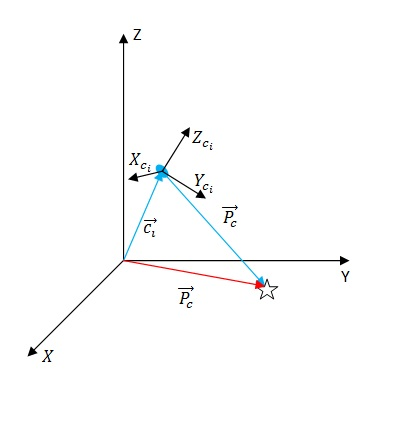
\includegraphics[width=0.5\linewidth]{../Images/c2/system_coordinates}
\caption[System Coordinates]{System Coordinates}
\label{fig:system_coordinates}
\end{figure}


%----------------------------------------------------------
\subsection{Camera Model}
	The model of the camera and its equations had been described on section 2.4. Matching Algorithm.
	
%----------------------------------------------------------
\subsection{Extended Kalman Filter}

The Kalman Filter is an iterative algorithm that obtain an estimation of a lineal dynamic system when sensors has white noise. In this case, the system is non-linear so it's used a variant called Extended Kalman Filter \cite{GabrielTerejanu} (or EKF ). To apply the algorithm it's necessary to use a linealization of the known system described previously. That means that to apply this EKF we consider only the cinematic (velocities of the objects to update their position).

\begin{equation}
P_{obj} = 
	\begin{pmatrix}
	x_k \\
	y_k \\
	z_k \\
	v^{x}_k \\
	v^{y}_k \\
	v^{z}_k \\
	\end{pmatrix}
=
	\begin{pmatrix}
	1 & 0 & 0 & \Delta{t} & 0 & 0 \\
	0 & 1 & 0 & 0 & \Delta{t} & 0 \\
	0 & 0 & 1 & 0 & 0 & \Delta{t} \\
	0 & 0 & 0 & 1 & 0 & 0 \\
	0 & 0 & 0 & 0 & 1 & 0 \\
	0 & 0 & 0 & 0 & 0 & 1 \\
	\end{pmatrix}
*
	\begin{pmatrix}
	x_{k-1} \\
	y_{k-1} \\
	z_{k-1} \\
	v^{x}_{k-1} \\
	v^{y}_{k-1} \\
	v^{z}_{k-1} \\
	\end{pmatrix}
\end{equation}

Consider the following nonlinear system described by the difference equation and the observation model with additive noise: \\

\begin{gather}
x_k = f(x_{k-1}) + w_{k-1} \\
z_k = h(x_k) + v_k
\end{gather}

Been $x_k$ the state of the system, $z_k$ the observation state, and $f(�) \& h(�)$ the functions of both systems with their noise $ w_k ; v_k$. \\
Every step of the EKF consist on two substeps called "Predictor" and "Corrector":

\begin{itemize}
   \item Predictor Step
		\begin{gather}
			x_k^{f} \approx f(x_{k-1}^{a}) \\
			P_k^{f} = J_f(x_{k-1}^{a}) P_{k-1} J_f^{T}(x_{k-1}^{a}) + Q_{k-1}
		\end{gather}

	\item CorrectorStep
		\begin{gather}
			P_k = (I - K_k J_h(x_k^{f}))P_k^{f} \\
			K_k = P_k^{f} J^{T}_h(x_k^{f}) (J_h(x_k^{f}) P_k^{f} J_h^{T}(x_k ^{f}) + R_k)^{-1} \\
			x_k^{a} \approx x_k^{f} + K_k (z_k - h(x_k^{f}))
		\end{gather}
\end{itemize}

In the previous ecuations, $J_h$ and $J_f$ are the Jacobian matrix of the system and observator. They are can be computed basing on the system and camera model as: \\

\[J_h =  
	\begin{pmatrix}
		\frac{\partial h_1}{\partial x_1} & \dots & \frac{\partial h_1}{\partial x_n} \\
		\vdots & \ddots & \vdots \\
		\frac{\partial h_m}{\partial x_1} & \dots & \frac{\partial h_m}{\partial x_n}
	\end{pmatrix}
\]

And so on with the $ f(�)$ function for the $J_f$ jacobian. Following paragraphs decribes the procedure of acquisition of both jacobians for this specific situation. \\

\begin{equation} \label{eq:observation_equation}
z_k =
	\begin{pmatrix}
		x_{img} \\
		y_{img}
	\end{pmatrix}
\stackrel{\ref{eq:pinhole_cam_eq}}{=}
	\begin{pmatrix}
		f*\frac{y_c}{x_c} \\
		f*\frac{z_c}{x_c}
	\end{pmatrix}
\end{equation}

Getting \ref{eq:system_equation} and isolating the position vector of the target in the camera's base, then is possible to express the observation state in term of real system state.

\begin{equation}
\ref{eq:system_equation} \Rightarrow 
	\begin{pmatrix}
		x_c \\
		y_c \\
		z_c 
	\end{pmatrix}
=
	\begin{pmatrix}
		r_{11} & r_{21} & r_{31} \\
		r_{12} & r_{22} & r_{32} \\
		r_{13} & r_{23} & r_{33}
	\end{pmatrix}
*
	\begin{pmatrix}
		x - c_x \\
		y - c_y \\
		z - c_z
	\end{pmatrix}
\end{equation}

So, individually:

\begin{equation}
\left\{ 
	\begin{split}
		x_c = r_{11}(x-c_x) + r_{21}(y-c_y) + r_{31}(z-c_z) \\
		y_c = r_{12}(x-c_x) + r_{22}(y-c_y) + r_{32}(z-c_z) \\
		z_c = r_{13}(x-c_x) + r_{23}(y-c_y) + r_{33}(z-c_z) 
	\end{split} \right.
\end{equation}

Introducing this in equation \ref{eq:observation_equation}.

\begin{equation}
z_k =
	\begin{pmatrix}
		-f�\frac{r_{11}(x-c_x) + r_{21}(y-c_y) + r_{31}(z-c_z)}{r_{13}(x-c_x) + r_{23}(y-c_y) + r_{33}(z-c_z)} \\
		f�\frac{r_{12}(x-c_x) + r_{22}(y-c_y) + r_{32}(z-c_z)}{r_{13}(x-c_x) + r_{23}(y-c_y) + r_{33}(z-c_z)}
	\end{pmatrix}
\end{equation}

This observation equation only includes information about one camera, since now, this section splits in two. The first one dedicated to stereo tracking with a pair of non-parallel cameras. And the second one, using only one camera but in order to reduce the number of variables (Unless the EKF will became unstable with this equations, in chapter \ref{chap:c6_conclusions} there is a dissertation about this topic). \\

%%% ------------------------------------------------------------------------------------------------
\subsubsection{Tracking of ground objects}
At this point, we suppose that in world coordinates the $z$ dimension of the target is constant, so the system state will be $x_k = (x, y, v_x, v_y)$. For this reason, $\partial z$ and $\partial v_z$ has no sense. Based on a lineal behavior in the system \ref{subsec:system_model} and on the observation equations \ref{eq:observation_equation}, the following matrix are the ones that define the EKF.

\begin{equation}
J_f = 
	\begin{pmatrix}
			1		&		0		&		\Delta_t	&		0					\\
			0		&		1		&		0					&		\Delta_t	\\
			0		&		0		&		1					&		0					\\
			0		&		0		&		0					&		1
	\end{pmatrix}
\end{equation}

\begin{equation}
J_h = 
	\begin{pmatrix}
		-\frac{r_{11}z_c - r_{13}x_c}{x_c^2} & -\frac{r_{21}z_c - r_{23}x_c}{z_c^2}  & 0 & 0  \\
		\frac{r_{12}z_c - r_{13}y_c}{x_c^2} & \frac{r_{22}z_c - r_{23}y_c}{z_c^2}  & 0 & 0 
	\end{pmatrix}
\end{equation}

Such that, $(x_c, y_c, z_c)$ are related to camera position ob the object, $r_ij$ means the $(i,j)$ element of the rotation matrix of the camera.\\ 

%%% ------------------------------------------------------------------------------------------------
\subsubsection{Stereo Tracking}
At this point, unlike previous section the target can move in three coordinates, so the system state will be $x_k = (x, y, z, v_x, v_y, v_z)$. Based on a lineal behavior in the system \ref{subsec:system_model} and on the observation equations \ref{eq:observation_equation}, the following matrix are the ones that define the EKF.

\begin{equation}
J_f = 
	\begin{pmatrix}
			1		&		0		&		0		&		\Delta_t	&		0					&		0					\\
			0		&		1		&		0		&		0					&		\Delta_t	&		0					\\
			0		&		0		&		1		&		0					&		0					&		\Delta_t	\\
			0		&		0		&		0		&		1					&		0					&		0					\\
			0		&		0		&		0		&		0					&		1					&		0					\\
			0		&		0		&		0		&		0					&		0					&		1
	\end{pmatrix}
\end{equation}

\begin{equation}
J_h = 
	\begin{pmatrix}
		-\frac{r_{11}^{c1}z^{c1}_c - r_{13}^{c1}x^{c1}_c}{{(z^{c1}_c)}^2} & -\frac{r_{21}^{c1}z^{c1}_c - r_{23}^{c1}x^{c1}_c}{{(z^{c1}_c)}^2} & -\frac{r_{31}^{c1}z^{c1}_c - r_{33}^{c1}x^{c1}_c}{{(z^{c1}_c)}^2} & 0 & 0 & 0 \\
		\frac{r_{12}^{c1}z_c^{c1} - r_{13}^{c1}y_c^{c1}}{{(z^{c1}_c)}^2} & \frac{r_{22}^{c1}z_c^{c1} - r_{23}^{c1}y_c^{c1}}{{(z^{c1}_c)}^2} & \frac{r_{32}^{c1}z_c^{c1} - r_{33}^{c1}y_c^{c1}}{{(z^{c1}_c)}^2} & 0 & 0 & 0 \\
		
		-\frac{r_{11}^{c2}z^{c2}_c - r_{13}^{c2}x^{c2}_c}{{(z^{c2}_c)}^2} & -\frac{r_{21}^{c2}z^{c2}_c - r_{23}^{c2}x^{c2}_c}{{(z^{c2}_c)}^2} & -\frac{r_{31}^{c2}z^{c2}_c - r_{33}^{c2}x^{c2}_c}{{(z^{c2}_c)}^2} & 0 & 0 & 0 \\
		\frac{r_{12}^{c2}z_c^{c2} - r_{13}^{c2}y_c^{c2}}{{(z^{c2}_c)}^2} & \frac{r_{22}^{c2}z_c^{c2} - r_{23}^{c2}y_c^{c2}}{{(z^{c2}_c)}^2} & \frac{r_{32}^{c2}z_c^{c2} - r_{33}^{c2}y_c^{c2}}{{(z^{c2}_c)}^2} & 0 & 0 & 0 \\
				
	\end{pmatrix}
\end{equation}

And as above, $(x_c, y_c, z_c)$ are related to camera position of the object, $r_ij$ means the $(i,j)$ element of the rotation matrix of the camera and $c_i$ superindex means related to camera i.
